\clearpage

\section{Binary Source}

\begin{tcolorbox}	
	\begin{tabular}{p{2.75cm} p{0.2cm} p{10.5cm}} 	
		\textbf{Header File}   &:& binary\_source\_*.h \\
		\textbf{Source File}   &:& binary\_source\_*.cpp \\
        \textbf{Version}       &:& 20180118 (Armando Pinto)\\
                               &:& 20180523 (Andr\'e Mourato)\\
                               &:& 20180815 (Andr\'e Mendes)
	\end{tabular}
\end{tcolorbox}

\maketitle
This block generates a sequence of binary values (1 or 0) and it can work in four\footnote{Modes \textit{AsciiFileAppendZeros} and \textit{AsciiFileCyclic} were removed and not implemented in the newer versions of LinkPlanner.} different modes:

\begin{multicols}{3}
\begin{enumerate}
	\item Random
	\item PseudoRandom
	\item DeterministicCyclic
	\item DeterministicAppendZeros
\end{enumerate}
\end{multicols}

\subsection*{Signals}

\begin{table}[h]
	\centering
	\begin{tabular}{|c|l|}
		\hline
		\textbf{Number of Input Signals} & 0 \\ \hline
        \textbf{Type of Input Signals} & - \\ \hline
    	\textbf{Number of Output Signals} & $\geq 1$ \ \\ \hline
        \textbf{Type of Output Signals} & Binary \\ \hline
	\end{tabular}
	\caption{Binary source signals}
	\label{table:bin_sour_signals}
\end{table}

\subsection*{Input Parameters}

\begin{table}[h]
	\centering
	\begin{tabular}{|c|c|p{60mm}|c|ccp{60mm}}
		\cline{1-4}
		\textbf{Parameter} & \textbf{Type} & \textbf{Values} &   \textbf{Default}& \\ \cline{1-4}
		mode & string & Random, PseudoRandom, DeterministicCyclic, DeterministicAppendZeros & PseudoRandom\\ \cline{1-4}
		probabilityOfZero & real & $\in$ [0,1] & 0.5 \\ \cline{1-4}
		patternLength & int &  Any natural number & 7 \\ \cline{1-4}
		bitStream & string & sequence of 0's and 1's & 0100011101010101 \\ \cline{1-4}
		numberOfBits & long int & any & -1 \\ \cline{1-4}
		bitPeriod & double & any & $1.0/100e9$ \\ \cline{1-4}
	\end{tabular}
	\caption{Binary source input parameters}
	\label{table:bin_sour_in_par}
\end{table}

\subsection*{Output Parameters}

\begin{table}[h]
	\centering
	\begin{tabular}{|c|c|p{60mm}|ccp{60mm}}
		\cline{1-3}
		\textbf{Parameter} & \textbf{Type} & \textbf{Values}& \\ \cline{1-3}
		Output Signal & string & sequence of 0's and 1's\\ \cline{1-3}
	\end{tabular}
	\caption{Binary source output parameters}
	\label{table:bin_sour_out_par}
\end{table}

\subsection*{Methods}

BinarySource(vector$\langle$Signal *$\rangle$ \&InputSig, vector$\langle$Signal *$\rangle$ \&OutputSig) :Block(InputSig, OutputSig)\{\};
\bigbreak	
void initialize(void);
\bigbreak	
bool runBlock(void);
\bigbreak
void setMode(BinarySourceMode m)
\bigbreak
BinarySourceMode const getMode(void)
\bigbreak	
void setProbabilityOfZero(double pZero)
\bigbreak
double const getProbabilityOfZero(void)
\bigbreak	
void setBitStream(string bStream)
\bigbreak
string const getBitStream(void)
\bigbreak	
void setNumberOfBits(long int nOfBits)
\bigbreak
long int const getNumberOfBits(void)
\bigbreak	
void setPatternLength(int pLength)
\bigbreak
int const getPatternLength(void)
\bigbreak	
void setBitPeriod(double bPeriod)
\bigbreak
double const getBitPeriod(void)

\subsection*{Functional description}

The \textit{mode} parameter allows the user to select between one of the four operation modes of the binary source.

\subparagraph*{Random Mode}
Generates a 0 with probability \textit{probabilityOfZero} and a 1 with probability (1-\textit{probabilityOfZero}).

\subparagraph*{Pseudorandom Mode}
Generates a pseudorandom sequence with period $2^\textit{patternLength}-1$.

\subparagraph*{DeterministicCyclic Mode}
Generates the sequence of 0's and 1's specified by \textit{bitStream} and then repeats it.

\subparagraph*{DeterministicAppendZeros Mode}
Generates the sequence of 0's and 1's specified by \textit{bitStream} and then it fills the rest of the buffer space with zeros.



\subsection*{Input Signals}


\subparagraph*{Number:} 0

\subparagraph*{Type:} Binary (DiscreteTimeDiscreteAmplitude)

\subsection*{Output Signals}

\subparagraph*{Number:} 1 or more

\subparagraph*{Type:} Binary (DiscreteTimeDiscreteAmplitude)

\subsection*{Illustrative Examples}

\paragraph*{Random Mode}
This mode generates a random sequence with \textit{patternLength}=3 which contains a total of 7 ($2^3-1$) bits. This sequence has an equal probability of generating 1's and 0's by default.

\pagebreak

\paragraph*{PseudoRandom Mode}
Consider a pseudorandom sequence with \textit{patternLength}=3 which contains a total of 7 ($2^3-1$) bits. In this sequence it is possible to find every combination of 0's and 1's that compose a 3 bit long subsequence with the exception of $000$. For this example the possible subsequences are $010$, $110$, $101$, $100$, $111$, $001$ and $011$ (they appear in figure \ref{BinarySequenceN3} numbered in this order).

\begin{figure}[H]
	\centering
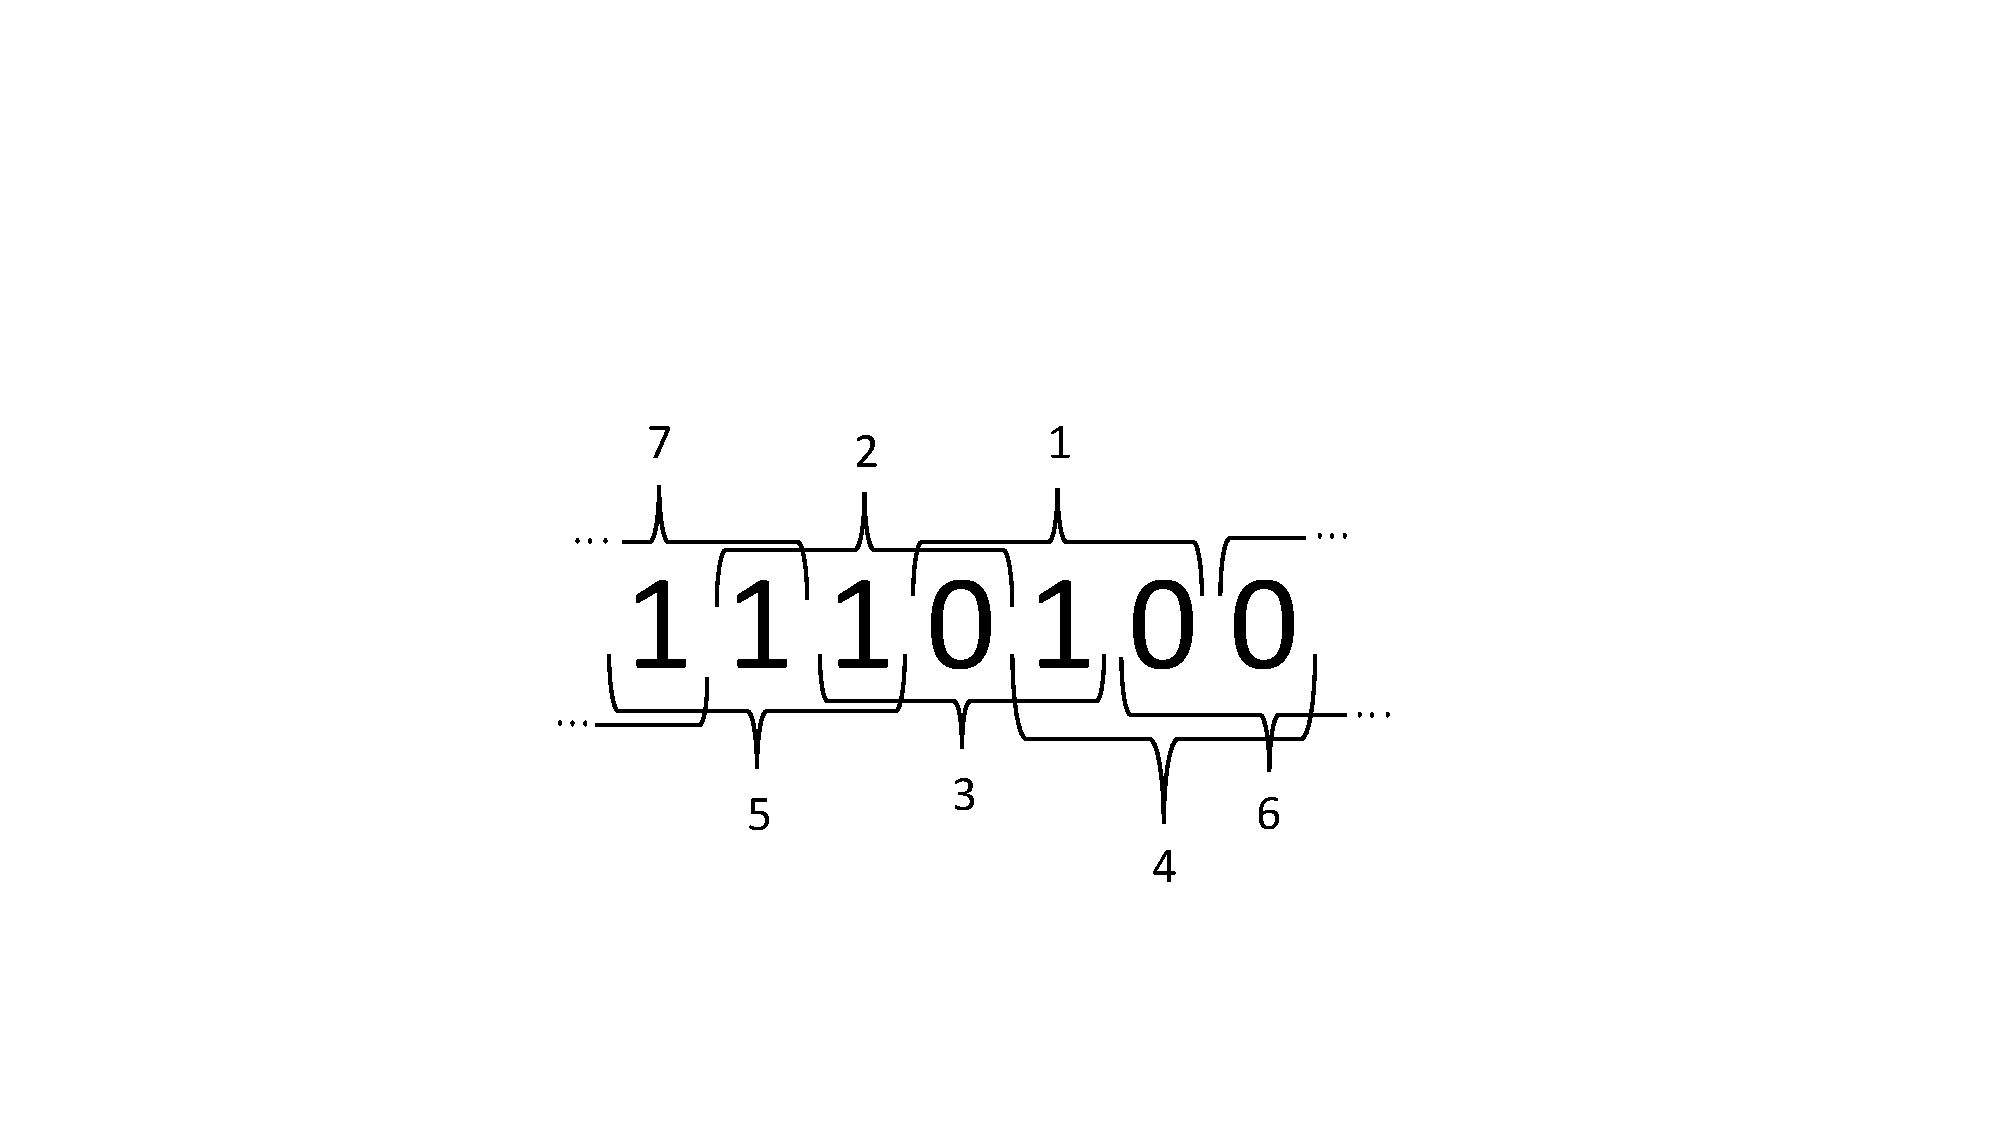
\includegraphics[width=\textwidth]{./lib/binary_source/figures/BinarySequenceN3.pdf}
\caption{Example of a pseudorandom sequence with a pattern length equal to 3.}\label{BinarySequenceN3}
\end{figure}

\pagebreak

\paragraph*{DeterministicCyclic Mode}

Take the \textit{bit stream} '0100011101010101'. In this case the sequence generated repeats $\frac{numberOfBits}{2^\textit{patternLength}-1}$ times. The generated binary signal is displayed in \ref{DeterministicCyclicSource}.

\begin{figure}[H]
	\centering
	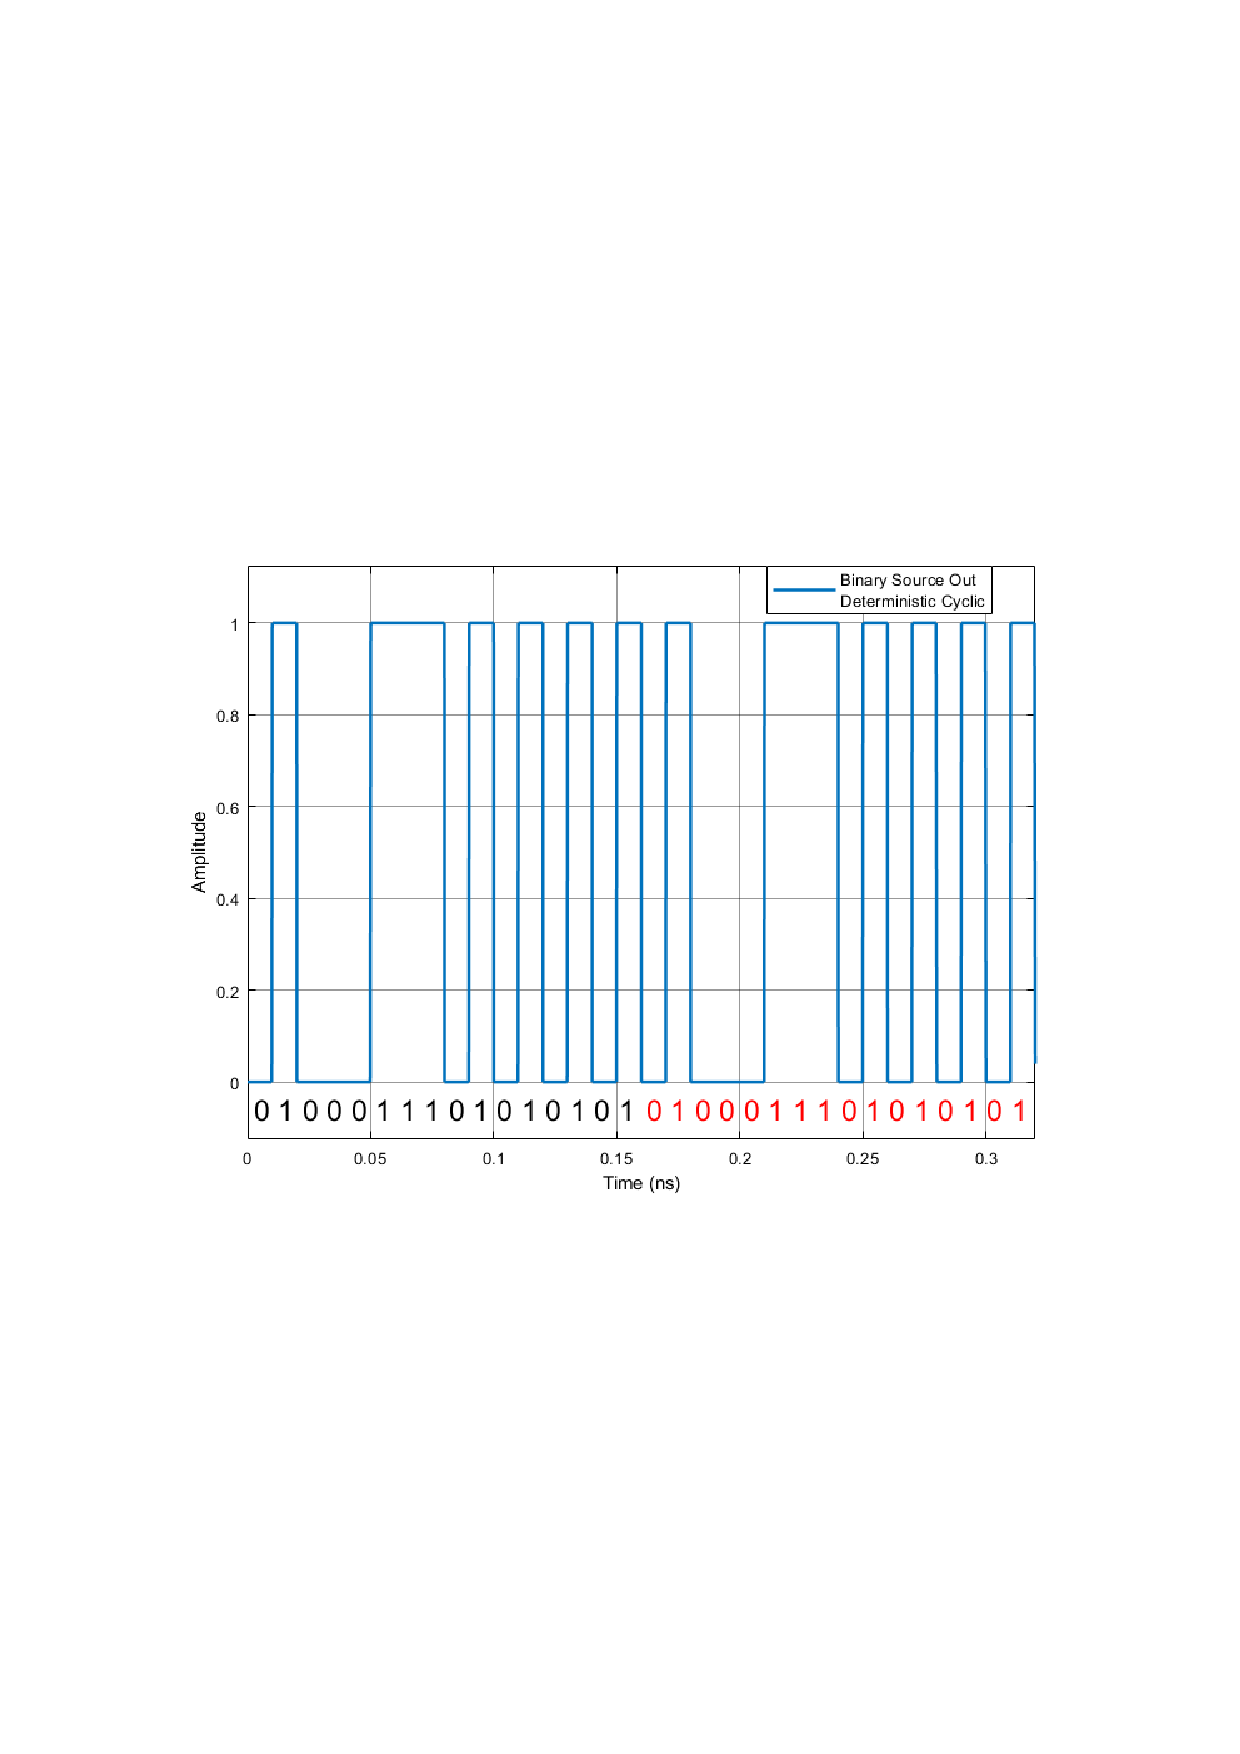
\includegraphics[clip, trim=0.5cm 9cm 0.5cm 9cm, width=\textwidth,scale=0.7]{./lib/binary_source/figures/BinarySource_output_Cyclic.pdf}
	
	\caption{Binary signal generated by the block operating in the \textit{Deterministic Cyclic} mode with a binary sequence 0100011101010101. In red is the repetition of the binary sequence.}\label{DeterministicCyclicSource}
\end{figure}

\pagebreak

\paragraph*{DeterministicAppendZeros Mode}

Take the \textit{bit stream} '0100011101010101'. After the \textit{bit stream} is generated the rest of the sequence is made of only 0's. The generated binary signal is displayed in \ref{DeterministicAppendZerosSource}.

\begin{figure}[H]
	\centering
	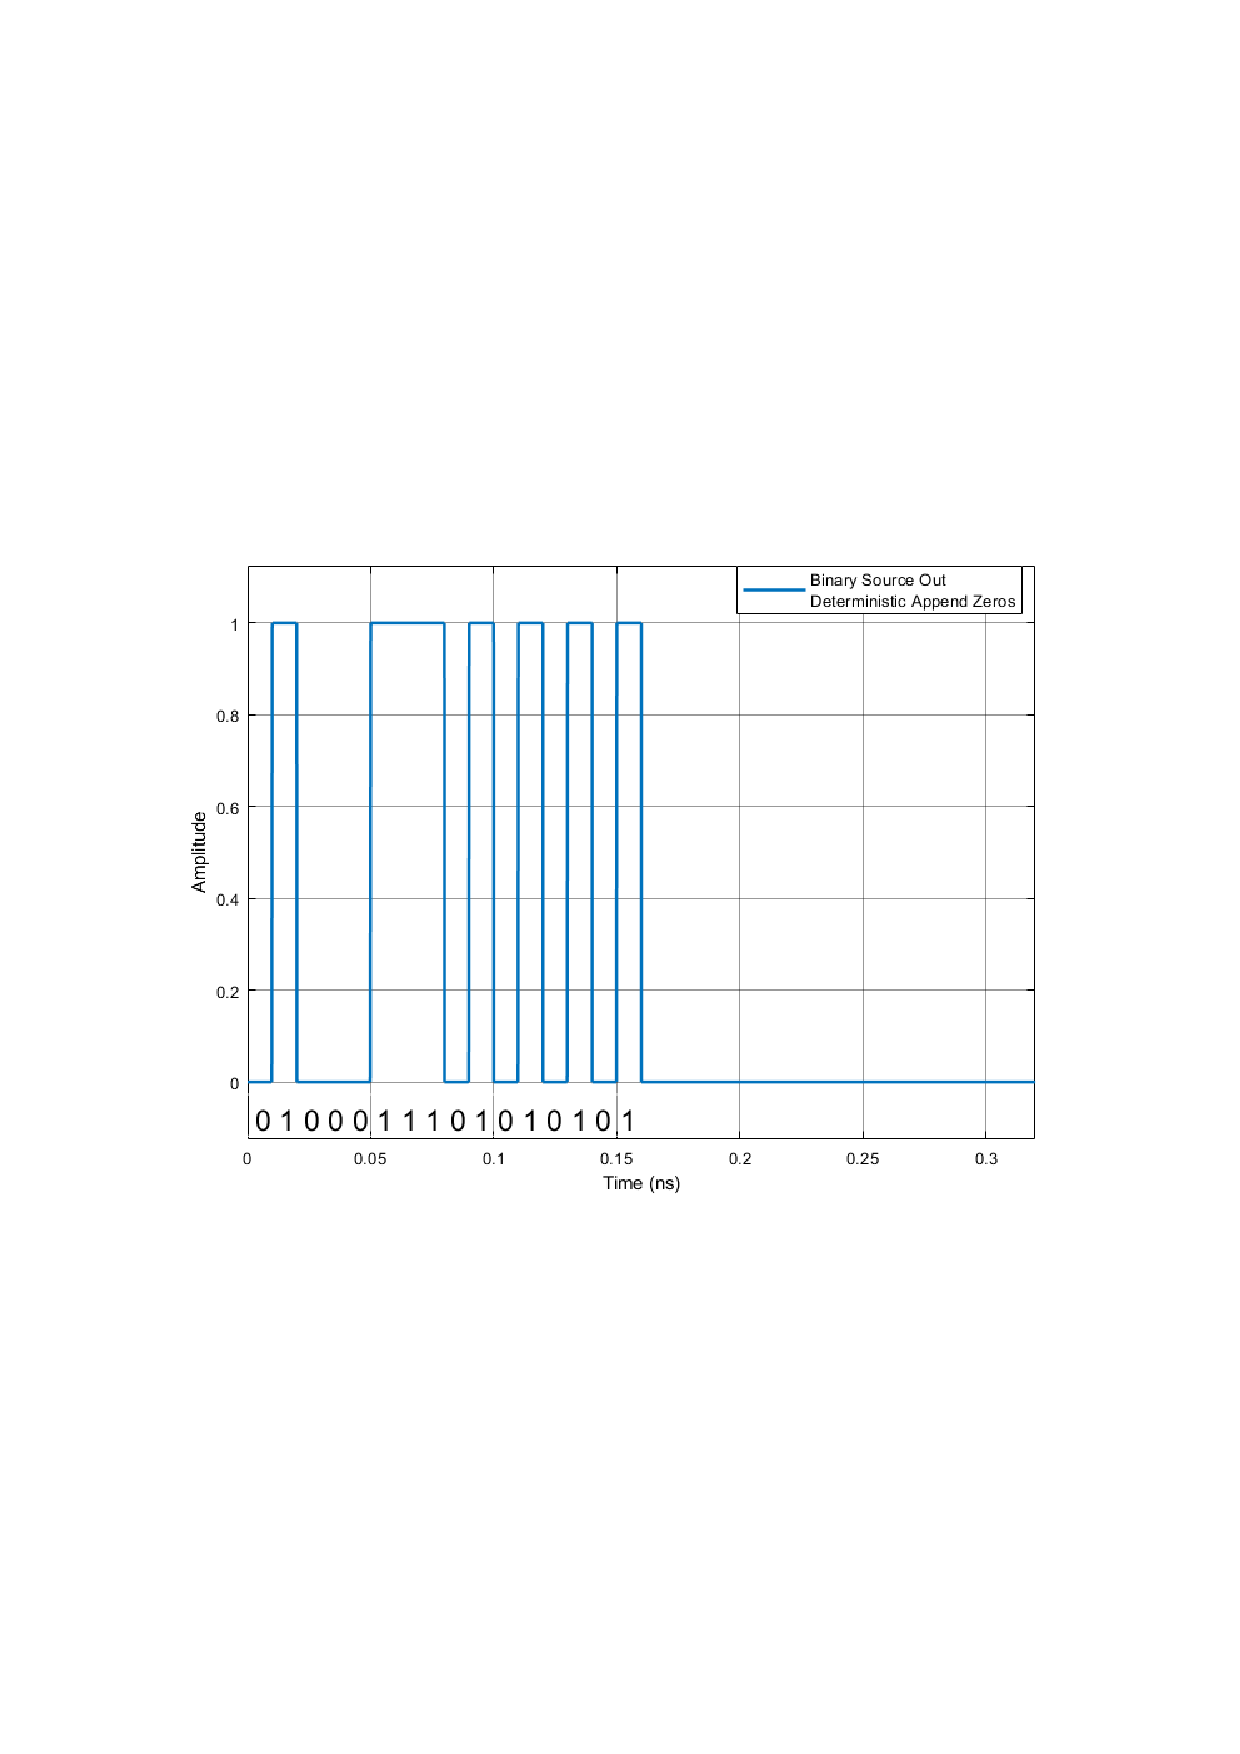
\includegraphics[clip, trim=0.5cm 9cm 0.5cm 9cm, width=\textwidth, scale=0.7]{./lib/binary_source/figures/BinarySource_output_appendZeros.pdf}
	
	\caption{Binary signal generated by the block operating in the \textit{Deterministic Append Zeros} mode with a binary sequence 0100011101010101.}\label{DeterministicAppendZerosSource}
\end{figure}

\subsection*{Suggestions for future improvement}

\indent Implement an input signal that can work as trigger.

Implement an input signal that can control the binary sequence generation mode.

Implement an input signal that can set the bitPeriod, therefore controlling the binary sequence rate.
